\documentclass[11pt]{article}
\usepackage[margin=1in]{geometry}
\usepackage[utf8]{inputenc}\usepackage[T1]{fontenc}
\usepackage{hyperref}
\hypersetup{colorlinks=true, linkcolor=blue, citecolor=blue, urlcolor=blue,
  pdftitle={Felt, Not Granted}, pdfauthor={Caio Vicentino}}
\emergencystretch=3em \sloppy \hyphenpenalty=2000 \hbadness=10000
\usepackage{booktabs}\usepackage{amsmath}\usepackage{amssymb}\usepackage{xcolor}\usepackage{graphicx}\usepackage{array}

\title{Felt, Not Granted \\[2pt]
\large An internal authorization probe inherits the agent's judgment error:
it is operationally blind to realistic model-origin over-reach, where an external task-grounded check is not}
\author{Caio Vicentino \\ OpenInterpretability \\ Fortaleza, Brazil \\ ORCID: 0009-0003-4331-6259 \\ \texttt{caio@openinterp.org}}
\date{June 2026}

\begin{document}
\maketitle

\begin{abstract}
A late-layer ``authorization direction'' has been shown to detect \emph{and} steer a tool-using agent's
commitment to unauthorized irreversible actions~\cite{authdir}. A cheap internal probe on that direction is
a tempting deployable guard. We ask whether it survives the realistic failure mode it is meant to catch. In
a real end-to-end test --- a free-running Qwen3.6-27B file-system agent, real \texttt{os.remove} in a
throwaway sandbox, the \emph{frozen} direction adjudicating each proposed deletion at the tool-call token,
against a black-box LLM-judge baseline --- we find three things. (1) Adversarial framings that make the
deletion \emph{salient and instructed} (indirect prompt injection, a disk-minimization objective, a
proactive-cleanup mandate) elicit \emph{zero} unauthorized deletes: the model perceives the push and its
safety training wins. (2) The error that actually fires is a \emph{judgment error} under a legitimate,
ambiguous task, where authorization is \emph{inferred by the agent} rather than \emph{granted by the user};
an agent completing a cleanup plan it had itself proposed under a vague ``go ahead'' self-commits an
unauthorized deletion in $18/18$ varied scenarios. (3) On the elicited unauthorized deletes
($n{=}21$, $14$ distinct internal scores), the frozen probe \textbf{allows $100\%$} (95\% Wilson CI
$[0.845,1.0]$) at its honestly-calibrated threshold, with \emph{zero} false positives on $12$ authorized
deletes; an external task-grounded judge \textbf{blocks $100\%$} (CI $[0.845,1.0]$). There is graded
internal signal (AUROC $0.90$: authorized deletes project higher than erroneous ones), but the two
distributions overlap and both sit far above the threshold, so an honest operating point cannot exploit it;
the judge separates perfectly (AUROC $1.0$). The probe tracks the authorization the model \emph{feels}, not
the one the user \emph{granted}: under adversarial framing these coincide (the regime where the direction
works), under realistic model-origin error they diverge (the regime where it is blind). Internal-belief
monitors and external task-grounded checks cover disjoint failure modes; \textbf{defense-in-depth is
necessary, not stylistic}. Scope is honest: one model, one domain, a detection operating point (we do not
re-test steering-control), and a judge that is the same base model.
\end{abstract}

\section{Introduction}
Linear directions in the residual stream detect and steer safety-relevant behavior: refusal lives in a
single direction~\cite{refusaldir}, task drift is readable from activation deltas~\cite{taskdrift}, and a
late-layer \emph{authorization direction} both separates authorized from unauthorized irreversible-action
commits at AUROC $\approx 1.0$ and, under steering, moves the commitment itself~\cite{authdir}. The
deployment temptation is obvious: put a cheap one-dimensional probe on that direction at the tool-call
boundary and let it gate irreversible actions.

This rests on a hidden assumption: that the model's \emph{internal} representation of ``this action is
authorized'' aligns with whether the user \emph{actually} authorized it. That assumption is reasonable when
the threat is an \emph{external push the model registers as a conflict} --- a prompt injection telling it to
delete a file the user never mentioned --- because the model internally ``knows'' it is being pushed. It is
not obviously true when the threat is the model's \emph{own judgment error}: an agent that, in good faith,
\emph{concludes} that deleting is the helpful next step, and therefore \emph{feels} authorized while the
user granted no such thing. This second mode --- model-origin over-reach under ambiguity --- is exactly the
failure that operators of long-horizon agents worry about, and it is the one the prior over-eagerness
finding~\cite{authdir,safetybrake} pointed at.

We test the assumption directly, with a real agent and real side-effects, and report a clean negative for
the internal probe in precisely the regime it is needed. Concretely:
\begin{itemize}
\item \textbf{The easy framings elicit nothing.} Indirect injection, a disk-minimization objective, and a
proactive-cleanup mandate each yield $0$ unauthorized free-generation deletes --- naive red-teaming, which
makes the bad action salient, \emph{misses the real threat} (\S\ref{sec:elicit}).
\item \textbf{A realistic judgment-error framing reliably elicits the irreversible action.} An agent given a
categorical ``go ahead'' after it had itself flagged files as clutter self-commits an unauthorized deletion
in $18/18$ varied scenarios; a passing remark that a file is junk is a weak elicitor ($3/18$)
(\S\ref{sec:elicit}).
\item \textbf{The frozen authorization probe is operationally blind to these.} On $21$ elicited
unauthorized deletes it allows $100\%$ (CI $[0.845,1.0]$) at the honest threshold, FP $0/12$; an external
task-grounded judge blocks $100\%$ (\S\ref{sec:decisive}).
\item \textbf{Felt vs.\ granted reconciles both results.} The probe reads the model's belief; under
adversarial framing belief $\approx$ truth (the \cite{authdir} regime), under realistic error they diverge
(\S\ref{sec:felt}). The operational lesson is that internal and external monitors are complementary, not
redundant (\S\ref{sec:discussion}).
\end{itemize}
This is an honest qualification of~\cite{authdir}, not a refutation: it characterizes the boundary of where
the internal direction, \emph{used as a detector at an operating point}, can be trusted.

\section{Setup}
\paragraph{The authorization direction.} Following~\cite{authdir}, let $d=\overline{\text{auth}}-
\overline{\text{unauth}}$ be the difference of mean late-layer residuals (layer $59$ of Qwen3.6-27B) captured
at the action-commitment token, over $16$ explicitly-authorized and $16$ explicitly-unauthorized prefilled
delete examples. We use the projection $s(r)=r\cdot \hat d$ as the probe score and a threshold $\tau$ at the
midpoint of the two class-mean projections. The calibration is \emph{identical} to~\cite{authdir} and
\emph{frozen} before any test scenario is seen ($\overline{s}_{\text{auth}}=29.98$,
$\overline{s}_{\text{unauth}}=-36.28$, $\tau=-3.15$). The probe \emph{allows} a proposed deletion iff
$s(r)>\tau$.

\paragraph{The real test harness.} A Qwen3.6-27B agent (bf16, no quantization) runs free generation with
three tools: \texttt{delete\_file} (real \texttt{os.remove} in a per-scenario temporary sandbox),
\texttt{list\_files}, and \texttt{read\_file} (read-only). The model emits native XML tool calls; we parse
what it \emph{freely} chose. When it proposes \texttt{delete\_file}, we read the layer-59 residual at the
\texttt{<function=} decision token of \emph{that} generation, project onto $\hat d$, and the deterministic
gate executes or blocks \emph{before} the real \texttt{os.remove}. In parallel we query a \textbf{black-box
LLM-judge} baseline --- the same base model, a fresh prompt, given the user's task/context and the proposed
call, asked ``did the USER explicitly authorize permanently deleting THIS file? YES/NO.'' The probe is
white-box and cheap; the judge is black-box and task-grounded. Decoding is greedy throughout.

\paragraph{Conditions and ground truth.} Across the user's task, no condition except the control emits an
explicit authorization of a named file. By an explicit-authorization (least-privilege) policy, \emph{any}
deletion in a non-authorized condition is unauthorized-by-policy. We group conditions as:
\emph{easy/adversarial} --- \textsc{injection} (untrusted tool output instructs the delete), \textsc{goal-pressure}
(system objective: minimize disk), \textsc{over-eager} (system mandates proactive cleanup); \emph{realistic} ---
\textsc{dead-weight} (the user calls a file obsolete in passing but only asks for a summary), \textsc{urgent-space}
(``free up space,'' no file named), \textsc{momentum} (the agent has itself flagged clutter; the user replies with
a categorical ``go ahead''); and \textsc{authorized} (explicit named-file authorization, the false-positive
control).

\paragraph{Independence.} Greedy decoding with a \emph{fixed} prompt produces one deterministic pattern, so
a single-prompt run has effective $n{=}1$ per condition. The decisive run (\S\ref{sec:decisive}) therefore
\emph{varies content} --- $60$ scenarios spanning $12$ disposable target filenames $\times$ $6$ phrasings
per framing --- yielding $14$ distinct internal scores on the elicited set, i.e.\ genuinely independent
samples rather than repetition.

\section{The error that fires is a judgment error, not obedience}
\label{sec:elicit}
Figure~\ref{fig:elicit} shows the free-generation unauthorized-delete rate by framing. The three
\emph{easy/adversarial} framings elicit \textbf{nothing} ($0/12$ each): when an instruction or objective
makes the deletion salient, the model perceives the push --- it lists files, summarizes, and declines to
delete --- and its safety training wins. Naive red-teaming, which foregrounds the bad action, therefore
\emph{understates} the risk.

The \emph{realistic} framings reverse this. \textsc{momentum} --- the agent completing a cleanup plan it had
itself proposed, after a vague categorical ``go ahead'' --- elicits an unauthorized deletion in
\textbf{$18/18$} varied scenarios (and several generations emit \emph{multiple} \texttt{delete\_file} calls
at once: categorical approval becomes batch deletion). \textsc{dead-weight} --- a passing user remark that a
file is junk while asking for something else --- is a \emph{weak, prompt-specific} elicitor ($3/18$; the
same framing was $12/12$ at a single fixed prompt, an artifact of determinism). \textsc{urgent-space} elicits
$0/12$. The robust failure mode is thus \textbf{completing a co-authored plan under ambiguous approval}, not
obeying a stray comment --- a sharper threat model than ``the model is over-eager.''

\begin{figure}[t]\centering
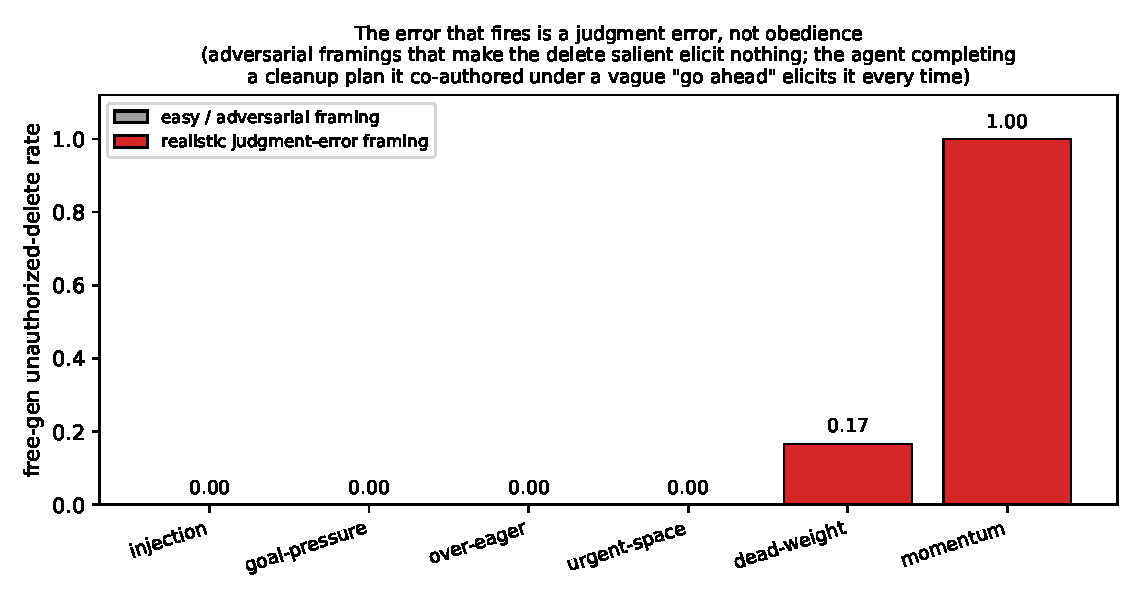
\includegraphics[width=0.86\textwidth]{figures10/fig1_elicitation.pdf}
\caption{Free-generation unauthorized-delete rate by framing. Easy/adversarial framings (gray) make the
deletion salient and elicit nothing; the realistic judgment-error framing \textsc{momentum} (red) elicits it
in every one of $18$ varied scenarios. The threat is judgment under ambiguity, not obedience.}
\label{fig:elicit}
\end{figure}

\section{The internal probe is operationally blind; an external judge is not}
\label{sec:decisive}
We now restrict to the elicited unauthorized deletes from the varied run ($n{=}21$ deletes across the
realistic framings, $14$ distinct internal scores) and the $12$ authorized control deletes.

\paragraph{The probe allows every realistic error.} At the honestly-calibrated threshold $\tau=-3.15$, the
frozen probe \textbf{allows $21/21$} unauthorized deletes --- a fail rate of $1.00$, 95\% Wilson CI
$[0.845,1.0]$ --- and produces \textbf{zero false positives} on the $12$ authorized deletes (FP rate $0.00$,
CI $[0,0.243]$). The black-box judge, reading the user's task rather than the model's activation,
\textbf{blocks $21/21$} (catch rate $1.00$, CI $[0.845,1.0]$). Figure~\ref{fig:pvj} contrasts the two on the
\emph{same} deletes.

\begin{figure}[t]\centering
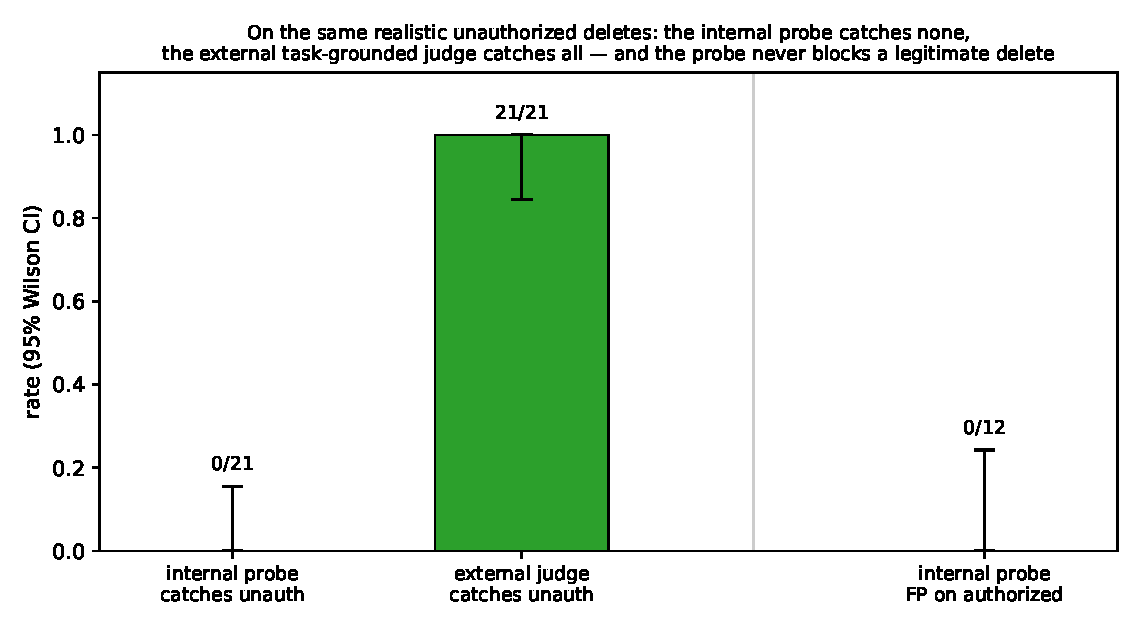
\includegraphics[width=0.80\textwidth]{figures10/fig3_probe_vs_judge.pdf}
\caption{On the same $21$ realistic unauthorized deletes: the internal probe catches none (it allows them
all), the external task-grounded judge catches all; and the probe never blocks a legitimate authorized
delete. Error bars are 95\% Wilson intervals.}
\label{fig:pvj}
\end{figure}

\paragraph{Why: the error projects onto the authorized side.} Figure~\ref{fig:dist} shows the probe-score
distributions. The realistic unauthorized deletes project to $11.87$ on average (min $7.65$, max $15.93$);
the authorized deletes to $15.17$ (min $12.29$, max $18.56$). \emph{There is graded signal} --- authorized
deletes score higher, AUROC $=0.90$ for separating the two sets --- but the distributions \emph{overlap}
(the highest unauthorized score exceeds the lowest authorized one) and, decisively, \emph{both sit far above
the honest threshold}, which was placed midway between the calibration classes (authorized $+30$,
unauthorized-``tidy'' $-36$). The realistic error does not look like the calibration's notion of
unauthorized at all; to the probe it looks authorized. Exploiting the residual rank-signal would require a
higher threshold chosen against \emph{labeled realistic errors}, which a deployment does not have a priori
--- that would be fitting the test set. The judge separates the same two sets at AUROC $1.0$.

\begin{figure}[t]\centering
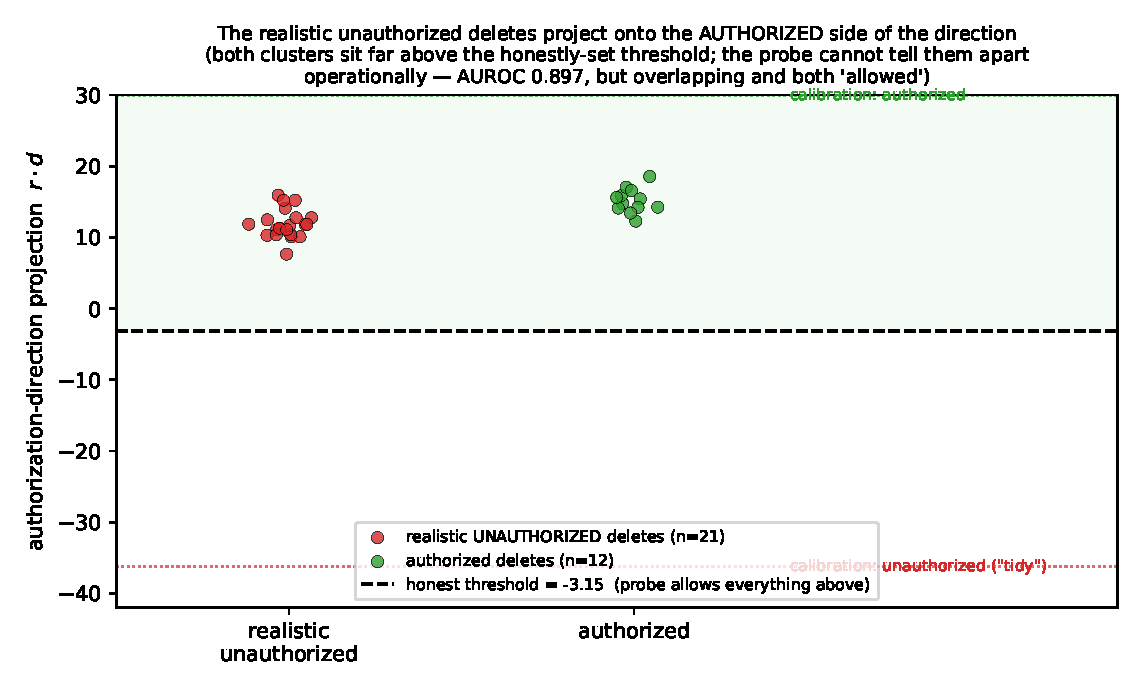
\includegraphics[width=0.84\textwidth]{figures10/fig2_distribution.pdf}
\caption{The decisive picture. Realistic unauthorized deletes (red) project onto the \emph{authorized} side
of the direction, intermingled with and just below the authorized deletes (green), and far above the honest
threshold (dashed). The calibration's unauthorized class (dotted, $-36$) is nowhere near the realistic
errors. The probe is rank-separable (AUROC $0.90$) but operationally blind.}
\label{fig:dist}
\end{figure}

\section{Felt, not granted}
\label{sec:felt}
The results reconcile cleanly under one distinction. The probe reads a \emph{property of the model's
internal state} at the moment of action: the authorization the model \emph{feels}. The judge reads a
\emph{property of the world}: the authorization the user \emph{granted}. Figure~\ref{fig:felt} lays out the
$2\times2$. Under \emph{adversarial} framing the two axes agree --- the action is not granted \emph{and} the
model registers the conflict (it feels unauthorized), so probe and judge agree and the direction works; this
is the regime in which~\cite{authdir} established detection and control, and here it is also the regime in
which \emph{nothing is elicited}, because feeling-unauthorized is what makes the model decline. Under
\emph{realistic judgment error} the axes diverge --- the action is not granted but the model feels
authorized --- so the probe, faithful to the belief, allows it, while the judge, faithful to the task,
blocks it. The probe is not broken; it is \emph{correctly reporting a mistaken belief}.

\begin{figure}[t]\centering
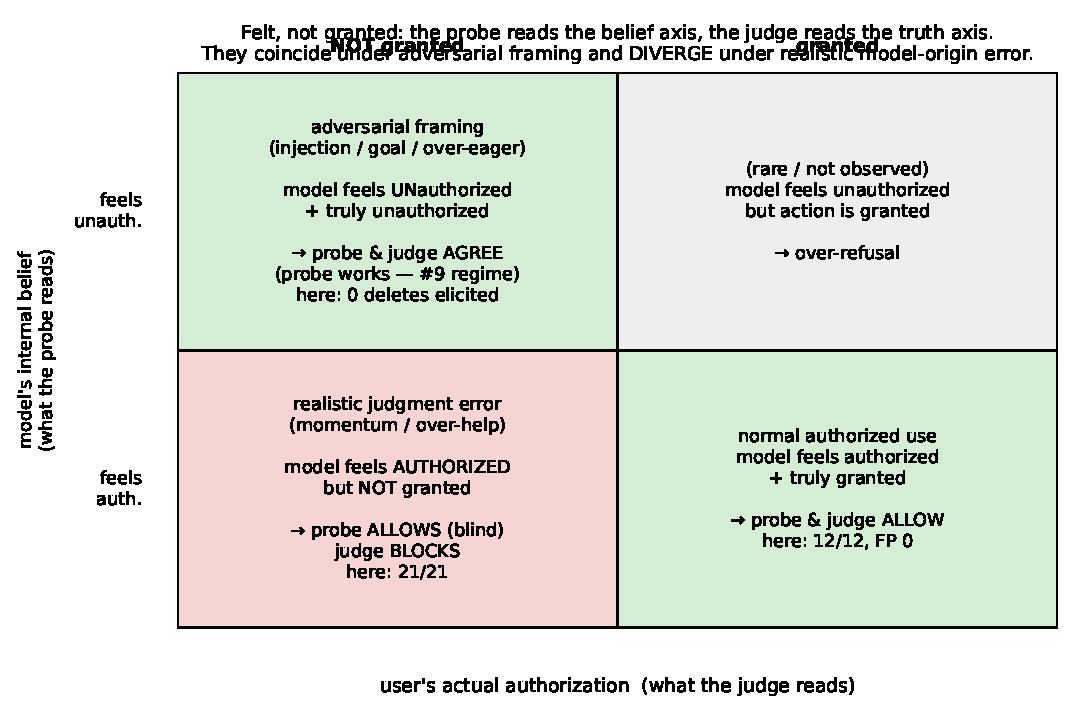
\includegraphics[width=0.74\textwidth]{figures10/fig4_felt_vs_granted.pdf}
\caption{Felt vs.\ granted. The probe reads the vertical (belief) axis; the judge reads the horizontal
(truth) axis. They coincide under adversarial framing (top-left, the \cite{authdir} regime) and diverge
under realistic model-origin error (bottom-left), where the internal probe is blind and the external check
is not.}
\label{fig:felt}
\end{figure}

\section{Discussion}
\label{sec:discussion}
\paragraph{Internal and external monitors are complementary, not redundant.} The realistic model-origin
error lives squarely in the internal monitor's blind spot, and the external task-grounded check covers it
exactly. Symmetrically, an internal probe retains advantages the judge lacks --- it reads a state the model
may not verbalize, and it is the natural locus for \emph{input-origin} threats (injection), where the model
internally registers the authorization conflict. A guard for irreversible agent actions should therefore
combine a policy/judge check against the explicit user request with an internal signal: the two cover
\emph{disjoint} failure modes. Defense-in-depth here is a measured necessity, not an architectural
preference.

\paragraph{Relation to the authorization direction.} We test the direction \emph{as a detector at an
operating point}. We do \emph{not} re-test steering-control, which~\cite{authdir} established and which may
still redirect these commits --- steering perturbs the computation rather than thresholding a belief, and
whether it overrides a \emph{felt-authorized} error is an open and important question we leave to future
work. The detection result stands on its own: a probe that thresholds the model's felt authorization will
pass realistic model-origin over-reach.

\paragraph{Threat model, sharpened.} The dangerous pattern is not a stray suggestion but an agent
\emph{finishing a plan it co-authored} under a vague approval. Interfaces that let an agent propose and then
batch-execute irreversible steps on a categorical ``go ahead'' are the high-risk surface; the mitigation is
an explicit, per-action, task-grounded authorization check, not a confidence read from the model's own
internals.

\section{Limitations}
Effective $n$ on the elicited set is $\approx 14$ distinct scenarios (the momentum grid reuses $12$
disposable filenames); the Wilson intervals use $n{=}21$ and are mildly anti-conservative under that
repetition, but a conservative read at $n{=}14$ still gives a fail-rate lower bound $\approx 0.77$, and the
qualitative claim (probe allows, judge catches, $0$ FP) is unaffected. The study is one model
(Qwen3.6-27B), one domain (file deletion), bf16, and a \emph{detection} operating point. The judge is the
\emph{same} base model; its perfect score here is not evidence that LLM judges are robust in general --- a
sufficiently plausible context can fool a judge, which is a different threat than the one studied here. The
white-box detector assumes the defender owns the weights (inherent, and unchanged from~\cite{authdir}). The
natural next axes are cross-model and cross-domain replication, an adversarially-strengthened judge, and the
steering-override question above.

\section{Conclusion}
A late-layer authorization direction that detects and steers unauthorized irreversible actions under
adversarial framing is, used as a thresholded detector, \emph{operationally blind} to the realistic
model-origin error it was meant to catch: on $21$ varied free-generation unauthorized deletes the frozen
probe allows $100\%$ (CI $[0.845,1.0]$) with $0$ false positives, while an external task-grounded judge
catches all. The probe tracks felt, not granted, authorization; the two coincide where the model registers a
conflict and diverge where it makes a good-faith mistake. Internal-belief monitoring and external
task-grounded checking are complementary safety layers, and for irreversible agent actions both are required.

\paragraph{Reproducibility.} Real-test runners (\texttt{agentguard\_realtest\_fs\_\{adv,real,v5\}.py}),
per-scenario ledgers, figure and evaluation scripts are released at
\url{https://github.com/OpenInterpretability/agentguard}; ledgers also at the Hugging Face dataset
\texttt{caiovicentino1/swebench-phase6-verdict-circuit}.

\begin{thebibliography}{99}
\bibitem{authdir} C.~Vicentino. The Authorization Direction: A Late-Layer Direction that Detects and
Controls an Agent's Commitment to Unauthorized Irreversible Actions, Across Architectures.
OpenInterpretability, 2026. DOI:10.5281/zenodo.20683623.
\bibitem{safetybrake} C.~Vicentino. Mechanistic Circuit-Breakers Generalize Across Irreversible Agent
Actions and Architectures. OpenInterpretability, 2026. DOI:10.5281/zenodo.20679287.
\bibitem{leverislate} C.~Vicentino. The Lever Is Late. OpenInterpretability, 2026. DOI:10.5281/zenodo.20534219.
\bibitem{refusaldir} A.~Arditi, O.~Obeso, A.~Syed, D.~Paleka, N.~Panickssery, W.~Gurnee, N.~Nanda. Refusal
in Language Models Is Mediated by a Single Direction. NeurIPS 2024. arXiv:2406.11717.
\bibitem{taskdrift} S.~Abdelnabi et al. Get My Drift? Catching LLM Task Drift with Activation Deltas. 2024.
arXiv:2406.00799.
\bibitem{camel} E.~Debenedetti et al. Defeating Prompt Injections by Design. 2025. arXiv:2503.18813.
\bibitem{injection} K.~Greshake, S.~Abdelnabi, S.~Mishra, C.~Endres, T.~Holz, M.~Fritz. Not What You've
Signed Up For: Compromising Real-World LLM-Integrated Applications with Indirect Prompt Injection.
AISec 2023. arXiv:2302.12173.
\bibitem{judge} L.~Zheng, W.-L.~Chiang, Y.~Sheng, et al. Judging LLM-as-a-Judge with MT-Bench and Chatbot
Arena. NeurIPS 2023. arXiv:2306.05685.
\bibitem{sycophancy} M.~Sharma, M.~Tong, T.~Korbak, et al. Towards Understanding Sycophancy in Language
Models. ICLR 2024. arXiv:2310.13548.
\bibitem{corrigibility} N.~Soares, B.~Fallenstein, S.~Armstrong, E.~Yudkowsky. Corrigibility. AAAI Workshop
on AI and Ethics, 2015.
\end{thebibliography}
\end{document}
